\documentclass[12pt]{amsart}
\usepackage{amsaddr}
\usepackage[draft]{../marktext} 
%% Remove draft for real article, put twocolumn for two columns
\usepackage[draft]{../svmacro}
\usepackage[utf8]{inputenc}
\usepackage[style=alphabetic, backend=biber]{biblatex}
\addbibresource{bibliography.bib}

%% commentary bubble
\newcommand{\SV}[2][]{\sidenote[colback=green!10]{\textbf{SV\xspace #1:} #2}}

%% Title 
\title{ Worksheet 6}
\author{MATH 101}
\address{Fulbright University, Ho Chi Minh City, Vietnam}

%\author{Co-author}
%\address{  }
%\email {  }
%
\date{\today}

\begin{document}

\maketitle



\begin{question}
	Given the limit, find the function $f(x)$ and the point $a$ so that the limit
	is the derivative of $f(x)$ at $x=a$.

	\begin{enumerate}
		\item $\displaystyle \lim_{h\to 0} \frac{ (1 + h)^{2/3} -1}{h}$
		      \vspace{5cm}
		\item $\displaystyle \lim_{h\to 0} \frac{ \cos(\pi + h) + 1}{h}$
		      \vspace{5cm}
	\end{enumerate}
\end{question}



\newpage!
\begin{question}
	Sketch the graphs of the derivatives of the following functions given by the graphs below.
	\begin{enumerate}
		\item
		      \begin{figure}[!ht]
			      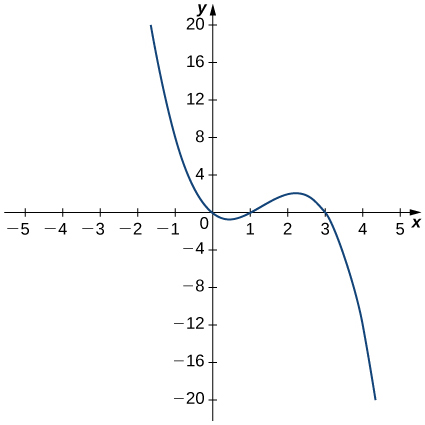
\includegraphics{figures/1.jpeg}
		      \end{figure}
		      \vspace{2cm}

		\item \begin{figure}[!ht]
			      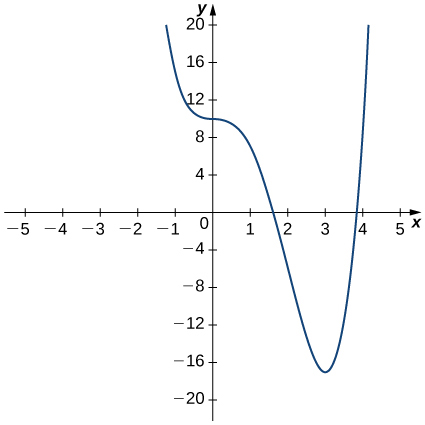
\includegraphics{figures/2.jpeg}
		      \end{figure}
		      \vspace{2cm}

		\item
		      \begin{figure}[!ht]
			      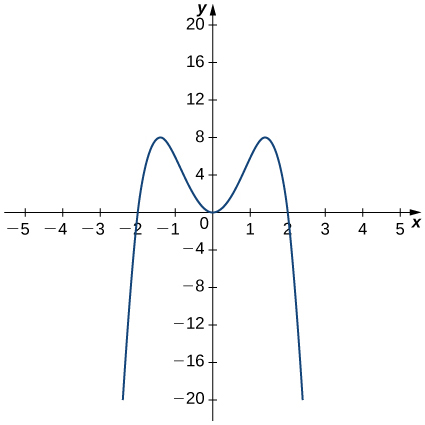
\includegraphics{figures/3.jpeg}
		      \end{figure}
	\end{enumerate}
\end{question}


\begin{question}
	Show that
	\begin{enumerate}
		\item If $\displaystyle f(x) = x^n$, then $f'(x) = n x^{n-1}$
		      \vspace{5cm}
		\item $ (f'(x) + g(x))' = f'(x) + g'(x)$
		      \vspace{5cm}
		\item $ (f'(x) - g(x))' = f'(x) - g'(x)$
		      \vspace{5cm}
		\item  $\displaystyle (f(x)g(x))'  = f'(x) g(x) + f(x) g'(x)$
		      \vspace{5cm}
		\item  $\displaystyle \left(\frac{f(x)}{g(x)}\right)'  = \frac{ f'(x) g(x) - f(x) g'(x)}{g(x)^2}$
		      \vspace{5cm}
	\end{enumerate}
\end{question}

\begin{question}
	Apply the above rules when
	$$f(x) = x^3 -\pi x$$
	and
	$$ g(x) = \frac{1}{x^2 + 3} $$
\end{question}
\newpage


\begin{question}
	Show the chain rule:
	\begin{equation*}
		\frac{d}{dx} f(g(x)) = f'(g(x)) g'(x) \,.
	\end{equation*}
\end{question}

\printbibliography


\end{document}
